\documentclass[12pt]{article}
\usepackage[utf8]{inputenc}
\usepackage{array}
\usepackage{xcolor}
\usepackage{graphicx}
\usepackage{mathtools}
\usepackage{amsmath}
\usepackage{multicol}
\usepackage{eqnarray}
\usepackage{wrapfig}


\usepackage{natbib}
\usepackage{hyperref}
\hypersetup{
	colorlinks=true,
	linkcolor=black,
	filecolor=mangeta,      
	urlcolor=blue,
	pdftitle={Overleaf Example},
	pdfpagemode=FullScreen,
}

\usepackage[margin=0.6in]{geometry}

\title{52nd—24th INTERNATIONAL-RUDOLF ORTVAY \\ PROBLEM SOLVING CONTEST IN PHYSICS \\ Problem 18}
\author{Nguyen Thanh Long}
\date{\today}

\begin{document}
	
\maketitle

\noindent We determine the coordinate of a point on conical shell with the spherical coordinate system $(r, \theta, \varphi)$ where $\theta = \arcsin \left( \frac{1}{\pi} \right) = const$, so we actually only need $(r, \varphi)$. Choose this coordinate system so that $\varphi = 0$ at $B$ and $\varphi = \pi$ at $C$.

\noindent With our coordinate system, if we let $j_{r}' = \frac{ j_{r} }{ \sin \theta } = \pi j_r$, the solution of this problem will be the same as when we consider a material of a large, thin, homogeneous metal plate.

\begin{center}
	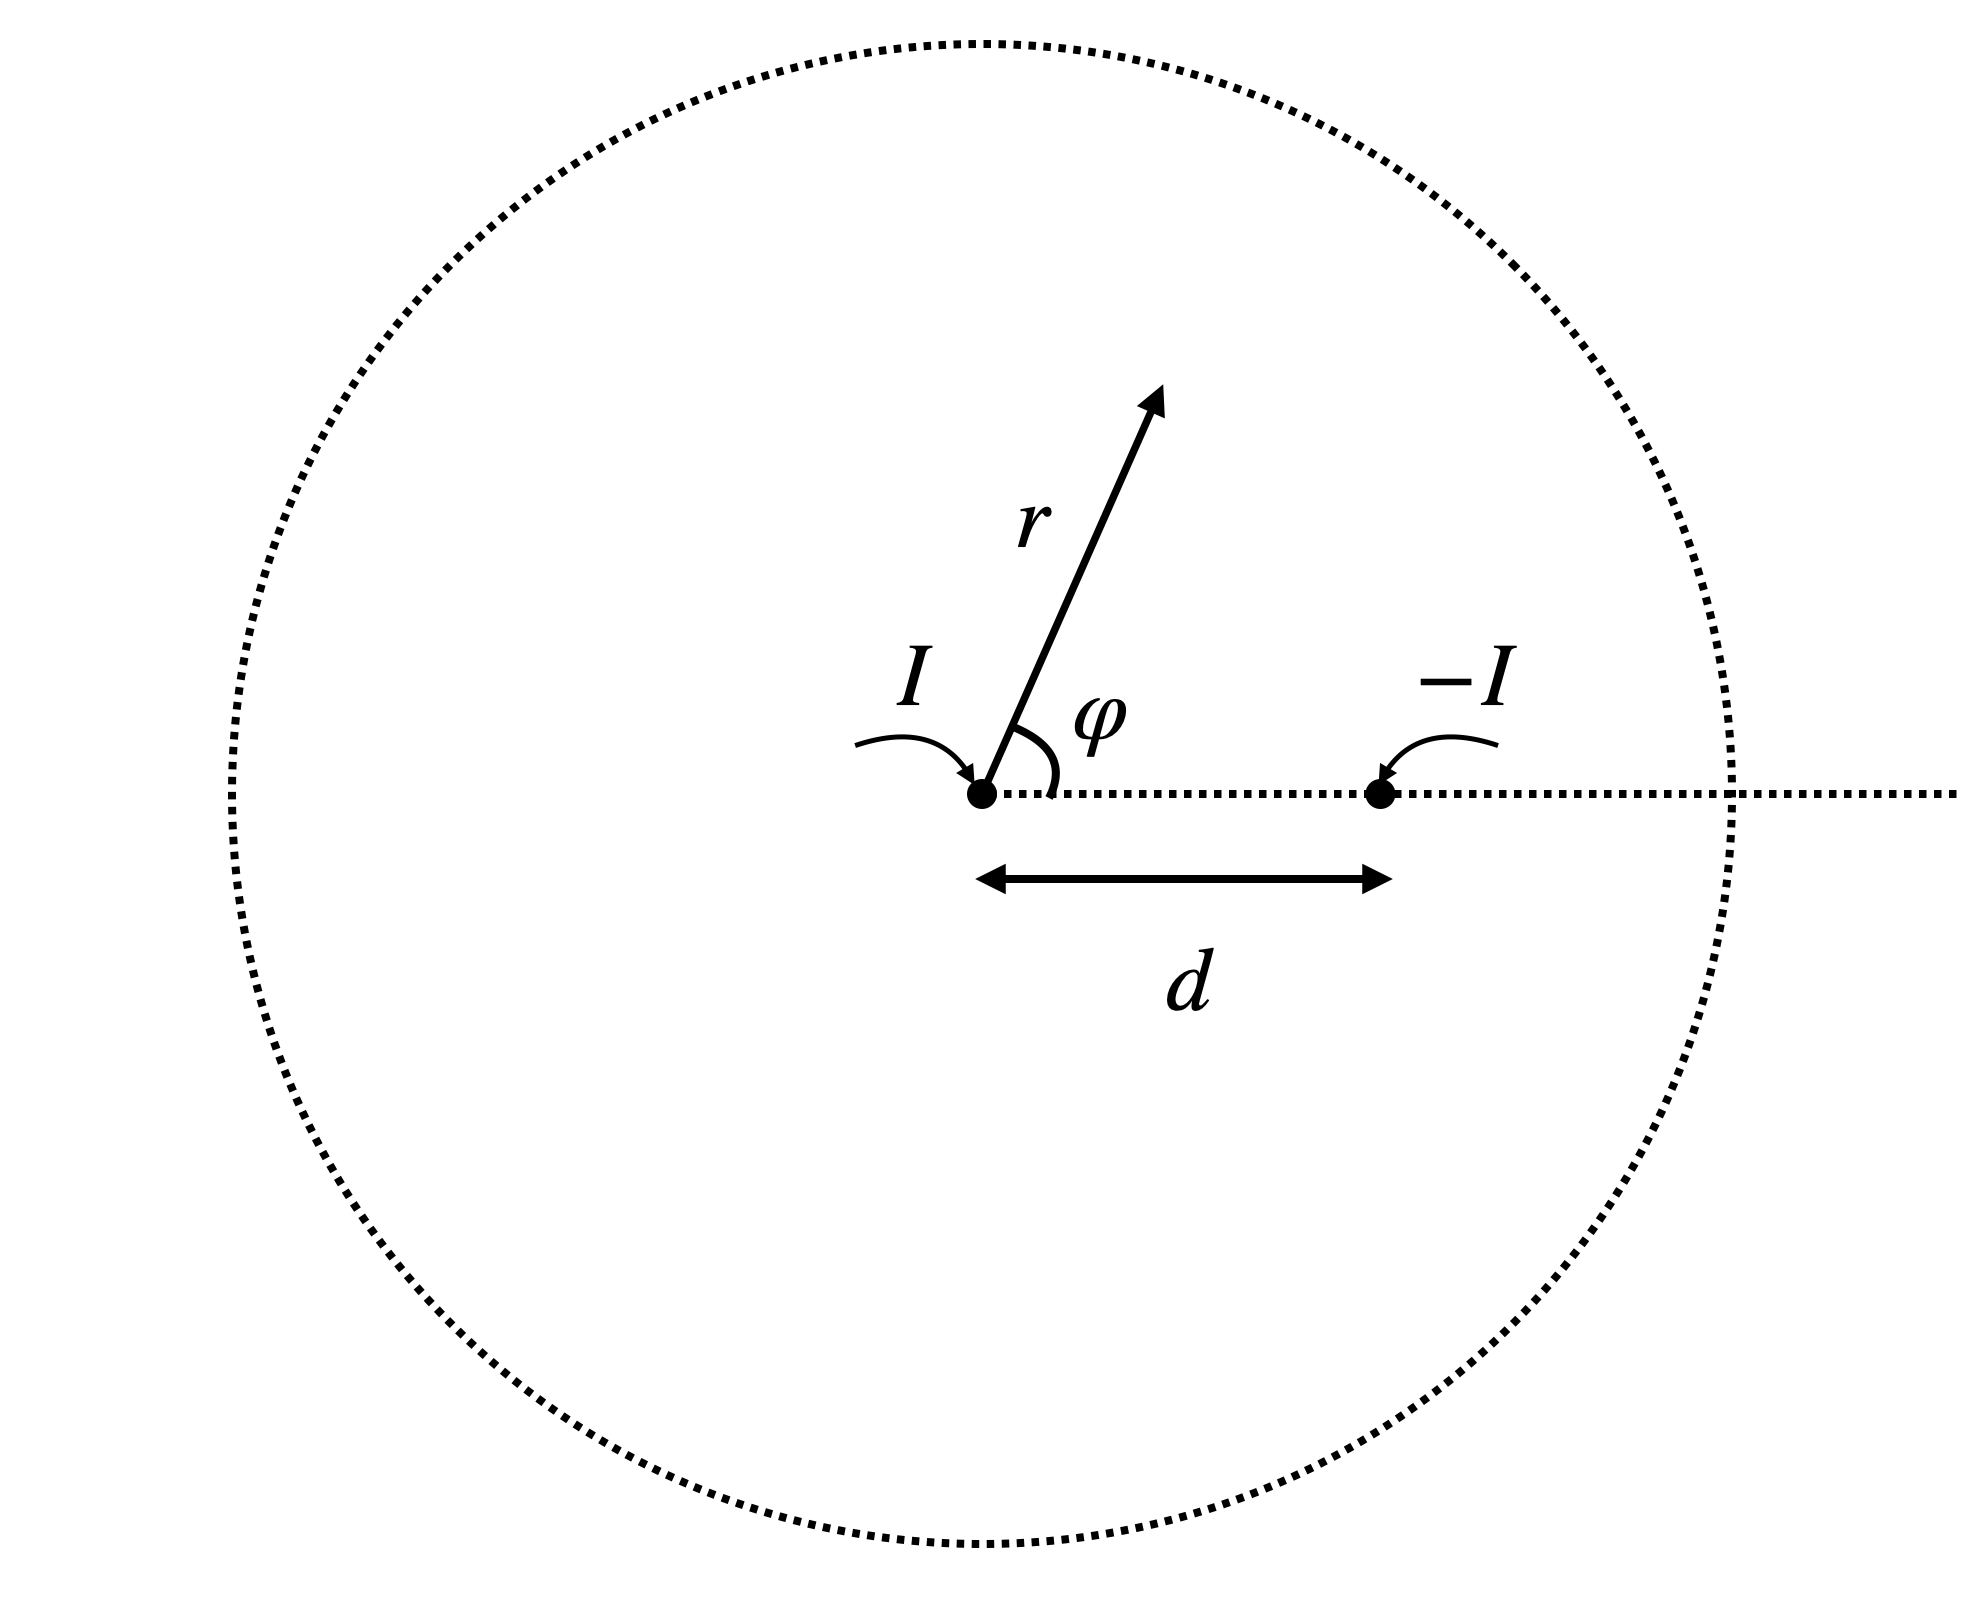
\includegraphics[width=0.6\textwidth]{Fig P18.png}
\end{center}	

\noindent In that case, we have:
\begin{align*}
	j_r' & = \frac{I}{2 \pi  \delta} \left( \frac{1}{r} - \frac{r - d \cos \varphi}{ d^2 + r^2 - 2 d r \cos \varphi } \right) . \\
	j_{\varphi} & = \frac{I}{2 \pi \delta} \frac{ d \sin \varphi }{d^2 + r^2 - 2 d r \cos \varphi} .
\end{align*}	
\noindent Return to our problem where $d = \pi R$, at $C$, $r = \pi R$ and $\varphi = \pi$ so the density current is: 
$$ j_C = \pi j_C' = \frac{I}{4 \pi \delta R} .$$
	
	
\end{document}